\chapter{Modelo Desenvolvido}
\label{cap:modelo}

\todo{revisar o conteúdo deste capítulo e ver se dá para desenvolver/detalhar melhor cada seção com infos do artigo, relatório e repositório}
\todo{escrever metodologia sobre o eixo de extensao tbm, e falar sobre o formulário}


Após a investigação do estado da arte em \textit{datasets} de tráfego DNS (Capítulo~\ref{cap:datasets}) e o estudo de redes neurais e de arquiteturas de IDS (Capítulos~\ref{cap:conceitos-basicos} e~\ref{cap:revisao-literatura}), o trabalho avançou para o desenvolvimento, treinamento e avaliação do modelo de classificação de tráfego DNS, cujos detalhes completos foram publicados no artigo~\citep{hirata2026dns} e cujo código está disponível no repositório do projeto\footnote{\url{https://github.com/giovannahirata/IDS-DNS}}.

\section**{Metodologia}

\todo{falar sobre metodologia para o eixo extensao: interação com publico externo, captura e analise de resultados}

A metodologia empregada seguiu as seguintes etapas: (i) revisão da literatura; (ii) decisão do modelo/arquitetura; (iii) pré-processamento dos dados (tratamento de \textit{features} categóricas, normalização de \textit{features} numéricas e remoção de \textit{features} com baixa variância ou que funcionam como identificadores); (iv) definição dos parâmetros e estrutura dos modelos; (v) treinamento; (vi) avaliação por meio de métricas de acurácia, precisão, recall e F1-\textit{score}; e (vii) interpretação dos resultados por meio da técnica de explicabilidade SHAP~\citep{lundberg2017}, que atribui a cada \textit{feature} um valor de contribuição para a decisão do modelo com base em teoria dos jogos, o que torna possível observar a contribuição de cada \textit{feature} para o modelo final decidir sobre o resultado mais provável. Para isso, o processo envolveu: treinar o modelo, usar a biblioteca SHAP para computar os valores SHAP, plotar esses valores e interpretar os resultados. Além disso, a biblioteca \textit{scikit-learn}~\citep{pedregosa2011} foi utilizada para os modelos clássicos, e a biblioteca TensorFlow~\citep{abadi2015} para a rede neural MLP.

Foram conduzidos experimentos de classificação binária (tráfego benigno vs. malicioso) e multiclasse (malware, phishing e spam, apenas entre as amostras malignas) com três algoritmos: SVM, KNN e MLP.

Todos os experimentos foram realizados em um computador equipado com um processador AMD Ryzen 9 7950X 16-Core e 128GB de RAM rodando o sistema operacional Debian Forky e o interpretador Python 3.13.11. Todos os códigos desenvolvidos para realização dos experimentos foram escritos em Python e estão disponíveis como \textit{software} livre\footnotemark[\value{footnote}].

\section**{Experimentos com o \textit{dataset} original}

Para o SVM, foram comparados os \textit{kernels} linear e RBF, variando os parâmetros de regularização $C$ e $\gamma$; devido à complexidade quadrática do \textit{kernel} RBF, seu treinamento foi limitado a 3.000 amostras. Para o KNN, o número de vizinhos $k$ foi variado entre 2 e 20. Para a MLP, foi utilizada uma arquitetura sequencial com camadas densas de 128, 64 e 32 neurônios (ativação ReLU), \textit{dropout} de 30\% entre camadas, otimizador Adam, \textit{early stopping} e redução da taxa de aprendizado no platô, treinada por 30 épocas, com saída \textit{sigmoid} (binário) ou \textit{softmax} (multiclasse). Sua arquitetura pode ser vista na Figura~\ref{fig:mlp-arquitetura}.

\begin{figure}[htb]
\centering
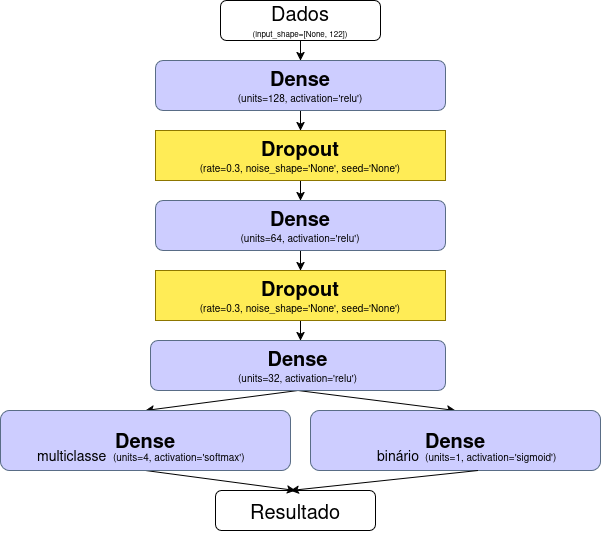
\includegraphics[width=.6\textwidth]{figuras/mlp-diagram.drawio.png}
\caption{Arquitetura do modelo MLP.}\label{fig:mlp-arquitetura}
\end{figure}

A Tabela~\ref{tab:resultados-original} resume as métricas obtidas por modelo no \textit{dataset} original (com todas as \textit{features}, incluindo \texttt{src\_port}):

\begin{table}[h]
    \centering
    \scriptsize
    \setlength{\tabcolsep}{3pt}
    \begin{tabular}{|l|c|c|c|c|r|}
    \hline
    \textbf{Algoritmo} & \textbf{Configuração} & \textbf{Acurácia} & \textbf{Precisão} & \textbf{Recall} & \textbf{F1-Score} \\ \hline
        SVM (binário)& SVC(kernel='linear', C=1) & 0,9917 & \textbf{1,0000} & 0,8072 & 0,8933 \\ \hline
        SVM (multiclasse)& SVC(kernel='rbf', C=10, gamma=0.01) & 0,8367 & 0,8394 & 0,8367 & 0,8266 \\ \hline
        KNN (binário) & n\_neighbors=3 & 0,9979 & 0,9652 & \textbf{0,9867} & \textbf{0,9758} \\ \hline
        KNN (multiclasse) & n\_neighbors=11 & 0,8925 & 0,8916 & 0,8925 & 0,8917 \\ \hline
        MLP (binário) & activation=`sigmoid’,loss=`binary\_crossentropy' & \textbf{0,9993} & 0,8541 & 0,9761 & 0,9111 \\ \hline
        MLP (multiclasse) & activation=`softmax’,loss=`sparse\_categorical\_crossentropy' & \textbf{0,9990} & \textbf{0,9993} & \textbf{0,9990} & \textbf{0,9991} 
        \\ \hline
    \end{tabular}
    \caption{Parâmetros e métricas de desempenho dos modelos.}
    \label{tab:resultados-original}
\end{table}

\section**{Descoberta de viés e engenharia de \textit{features}}

A análise de explicabilidade com SHAP revelou que, para os três algoritmos, a \textit{feature} \texttt{src\_port} (porta de origem) era, isoladamente, a mais influente para a decisão dos modelos, muito acima das demais, conforme ilustrado na Figura~\ref{fig:shap-antes}. A investigação da ferramenta de extração de fluxos utilizada na construção do \textit{dataset} (ALFlowLyzer~\citep{shafi2024a}) mostrou que a porta de origem é apenas um artefato do ambiente controlado em que o tráfego foi gerado, associada de forma acidental a cada categoria (por exemplo, \texttt{malware} e \texttt{phishing} sempre com a porta 46177), e não a uma característica real do comportamento do tráfego DNS. Ou seja, os modelos haviam aprendido um atalho estatístico do ambiente de geração do \textit{dataset}, e não um padrão de ataque generalizável.

\begin{figure}[h]
\centering
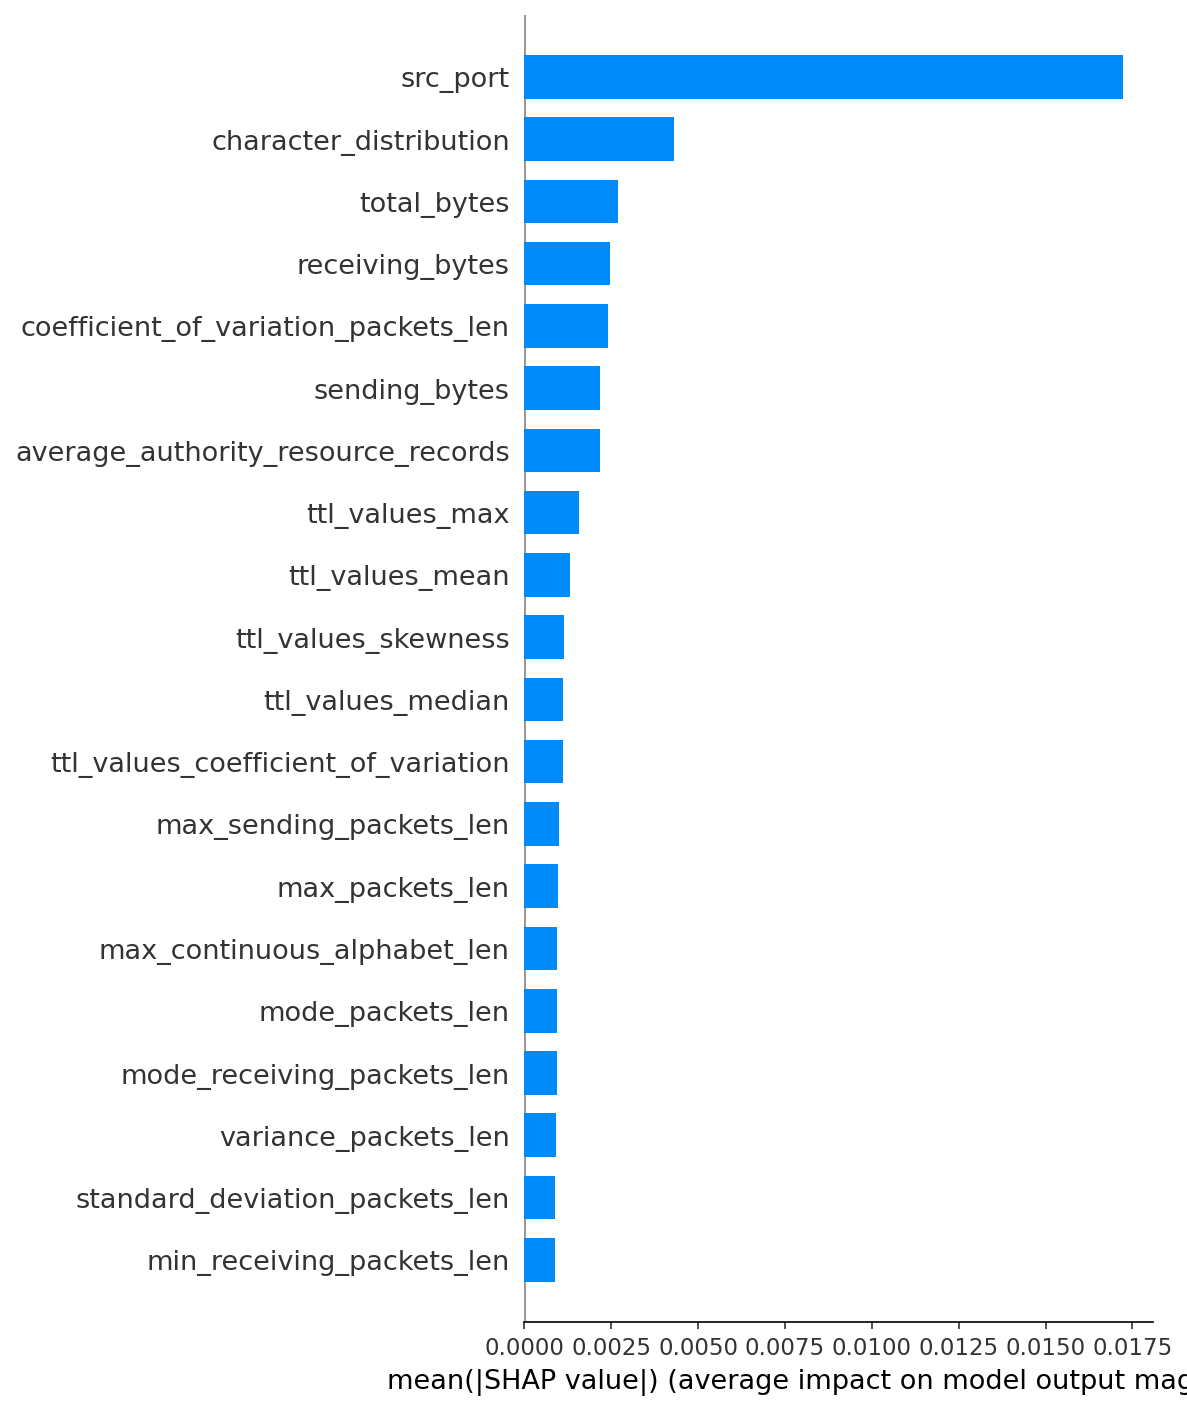
\includegraphics[width=0.75\textwidth]{figuras/shap_bar_plot_antes.png}
\caption{Importância das \textit{features} (SHAP) antes da remoção da \texttt{src\_port} -- modelo internacional.}
\label{fig:shap-antes}
\end{figure}

Diante dessa descoberta, um dos principais achados metodológicos do projeto, a \textit{feature} \texttt{src\_port} foi removida e todos os experimentos foram repetidos, priorizando as \textit{features} que efetivamente descrevem o comportamento do tráfego DNS (estatísticas de TTL, tamanho e taxa de pacotes, entropia e distribuição de caracteres do nome de domínio, entre outras). A Tabela~\ref{tab:resultados-sem-porta} resume os resultados obtidos sem a \texttt{src\_port}, e a Figura~\ref{fig:shap-depois} apresenta a nova ordem de importância das \textit{features} obtida por SHAP após essa remoção.

\begin{table}[h]
\centering
\caption{Desempenho dos modelos sem a \textit{feature} \texttt{src\_port}}
\label{tab:resultados-sem-porta}
\begin{tabular}{lcccc}
\toprule
Modelo (tarefa) & Acurácia & Precisão & Recall & F1-Score \\
\midrule
SVM (binário) & 0,7721 & 0,1203 & 0,6782 & 0,2044 \\
SVM (multiclasse) & 0,7170 & 0,7294 & 0,7170 & 0,7116 \\
KNN (binário) & 0,9704 & 0,7042 & 0,5427 & 0,6130 \\
KNN (multiclasse) & 0,8656 & 0,8652 & 0,8656 & 0,8642 \\
MLP (binário) & 0,9964 & 0,4924 & 0,7698 & 0,6006 \\
MLP (multiclasse) & 0,9966 & 0,9972 & 0,9966 & 0,9968 \\
\bottomrule
\end{tabular}
\end{table}

\begin{figure}[h]
\centering
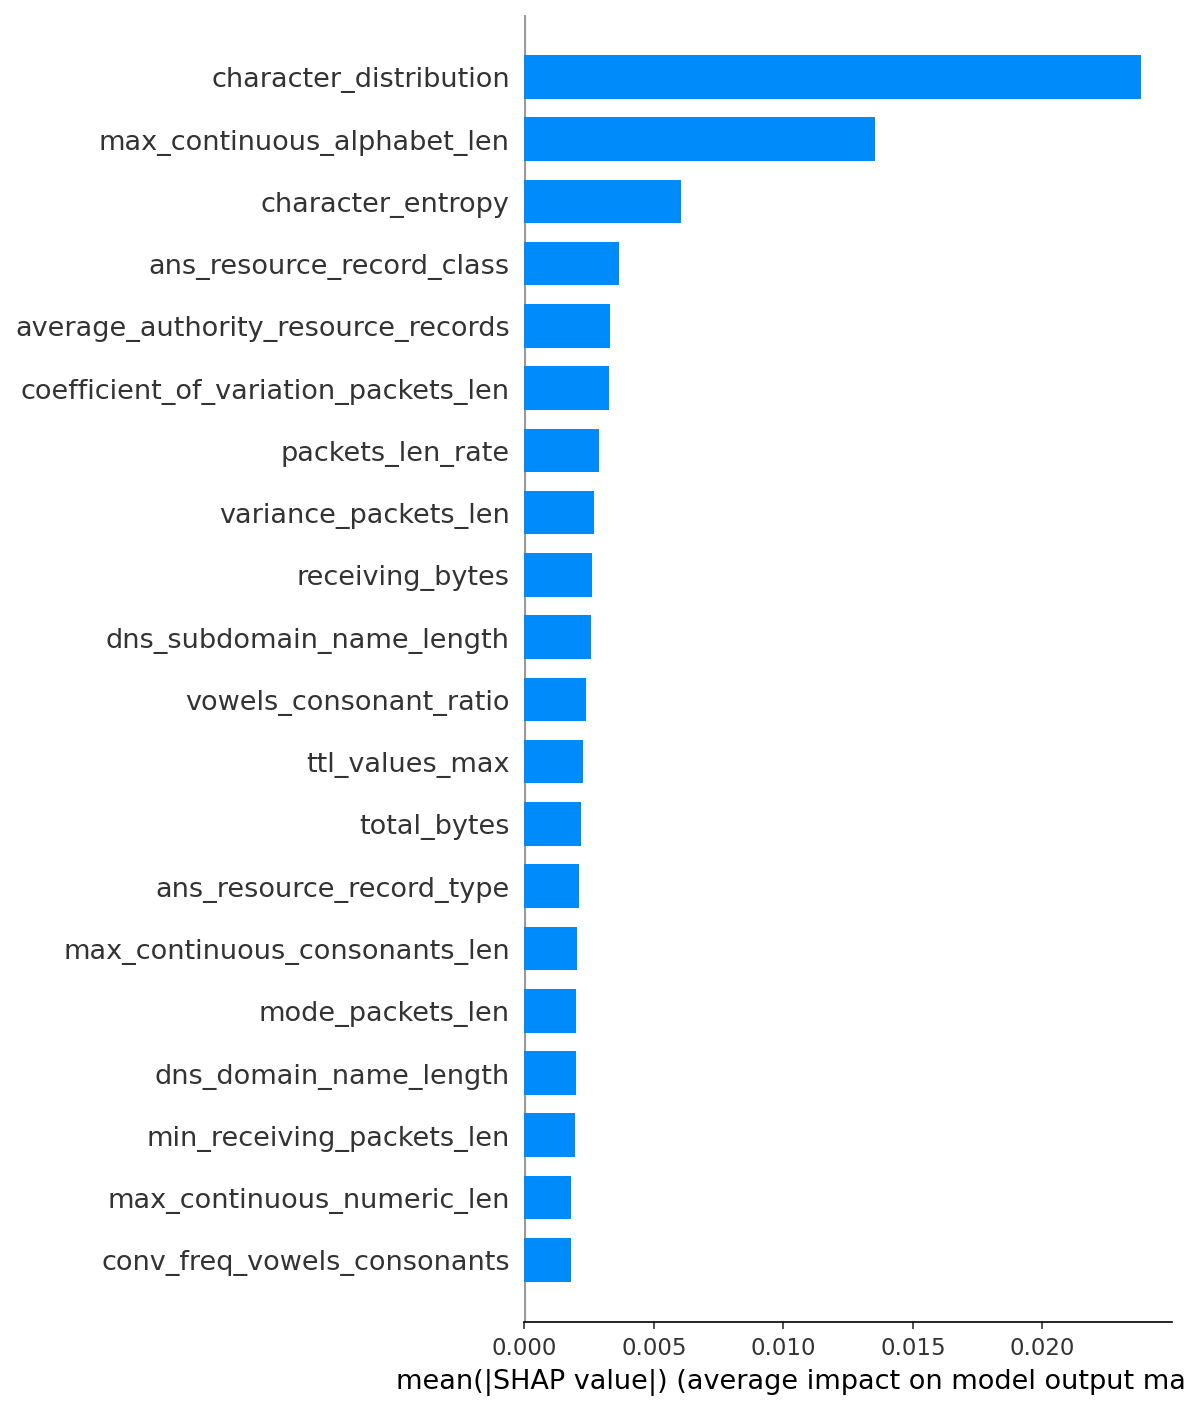
\includegraphics[width=0.75\textwidth]{figuras/shap_bar_plot_depois_sem_src_port.png}
\caption{Importância das \textit{features} (SHAP) depois da remoção da \texttt{src\_port}, sem balanceamento -- modelo internacional.}
\label{fig:shap-depois}
\end{figure}

Os resultados mostram que SVM e KNN foram fortemente prejudicados pela remoção da \texttt{src\_port}, confirmando que seu bom desempenho anterior era artificial. Já a MLP multiclasse manteve desempenho elevado e estável; a MLP binária, por sua vez, teve queda expressiva de precisão (de 0,8541 para 0,4924) em relação ao \textit{dataset} original, indicando que também a MLP binária dependia parcialmente da \texttt{src\_port} para seu desempenho, ainda que em menor grau do que SVM e KNN. A MLP multiclasse, portanto, manteve seu desempenho elevado, o que a tornou o modelo mais indicado para compor o mecanismo de detecção proposto.


\section**{Balanceamento de classes}

Como o \textit{dataset} é fortemente desbalanceado (mais de 95\% de amostras benignas), o que penaliza a detecção das classes minoritárias, especialmente \textit{spam}, foi conduzido um experimento de balanceamento: para cada uma das 10 repetições, foi selecionado aleatoriamente um subconjunto de amostras benignas de tamanho igual à soma de todas as amostras malignas (sem descartar nenhuma amostra maliciosa), seguido da divisão 70/30 entre treino e teste. As Tabelas~\ref{tab:mlp-bin-class} e ~\ref{tab:mlp-multi-class} apresentam o desempenho do modelo MLP, por classe, após treinamento (São apresentadas as médias das métricas e os desvios padrão considerando as 10 repetições). O modelo MLP multiclasse, treinado sobre o \textit{dataset} balanceado, obteve acurácia de 0,8819, precisão de 0,8808, recall de 0,8819, F1-\textit{score} de 0,8813 e AUC-ROC de 0,9792, com ganhos expressivos de recall para as classes minoritárias (malware, phishing e spam) em relação ao cenário desbalanceado, ao custo de uma acurácia geral mais baixa, o que consiste em uma troca considerada adequada para um sistema de detecção de intrusão, no qual minimizar falsos negativos é mais crítico do que maximizar a acurácia bruta. A Figura~\ref{fig:shap-balanceado} apresenta a importância das \textit{features} (SHAP) para esse modelo balanceado, mantendo o mesmo padrão observado na Figura~\ref{fig:shap-depois}, liderado por \texttt{character\_distribution}.


\begin{table}[H]
\centering
\caption{Desempenho da arquitetura MLP na classificação binária.}\label{tab:mlp-bin-class}
\begin{tabular}{lccc}
\toprule
Classe & Precisão média $\pm$ dp & Recall médio $\pm$ dp & F1-score médio $\pm$ dp \\
\midrule
Benigno   & 0,9455 $\pm$ 0,0037 & 0,9535 $\pm$ 0,0049 & 0,9495 $\pm$ 0,0015 \\
Malicioso & 0,9532 $\pm$ 0,0046 & 0,9450 $\pm$ 0,0042 & 0,9491 $\pm$ 0,0014 \\
\bottomrule
\end{tabular}
\end{table}

\begin{table}[H]
\centering
\caption{Desempenho da arquitetura MLP na classificação multiclasse.}\label{tab:mlp-multi-class}
\begin{tabular}{lccc}
\toprule
Classe & Precisão média $\pm$ dp & Recall médio $\pm$ dp & F1-score médio $\pm$ dp \\
\midrule
Benigno  & 0,9423 $\pm$ 0,0071 & 0,9645 $\pm$ 0,0049 & 0,9532 $\pm$ 0,0025 \\
Malware  & 0,8199 $\pm$ 0,0140 & 0,8357 $\pm$ 0,0165 & 0,8275 $\pm$ 0,0073 \\
Phishing & 0,8637 $\pm$ 0,0227 & 0,7961 $\pm$ 0,0231 & 0,8283 $\pm$ 0,0165 \\
Spam     & 0,8396 $\pm$ 0,0213 & 0,7864 $\pm$ 0,0241 & 0,8119 $\pm$ 0,0172 \\
\bottomrule
\end{tabular}
\end{table}

\begin{figure}[h]
\centering
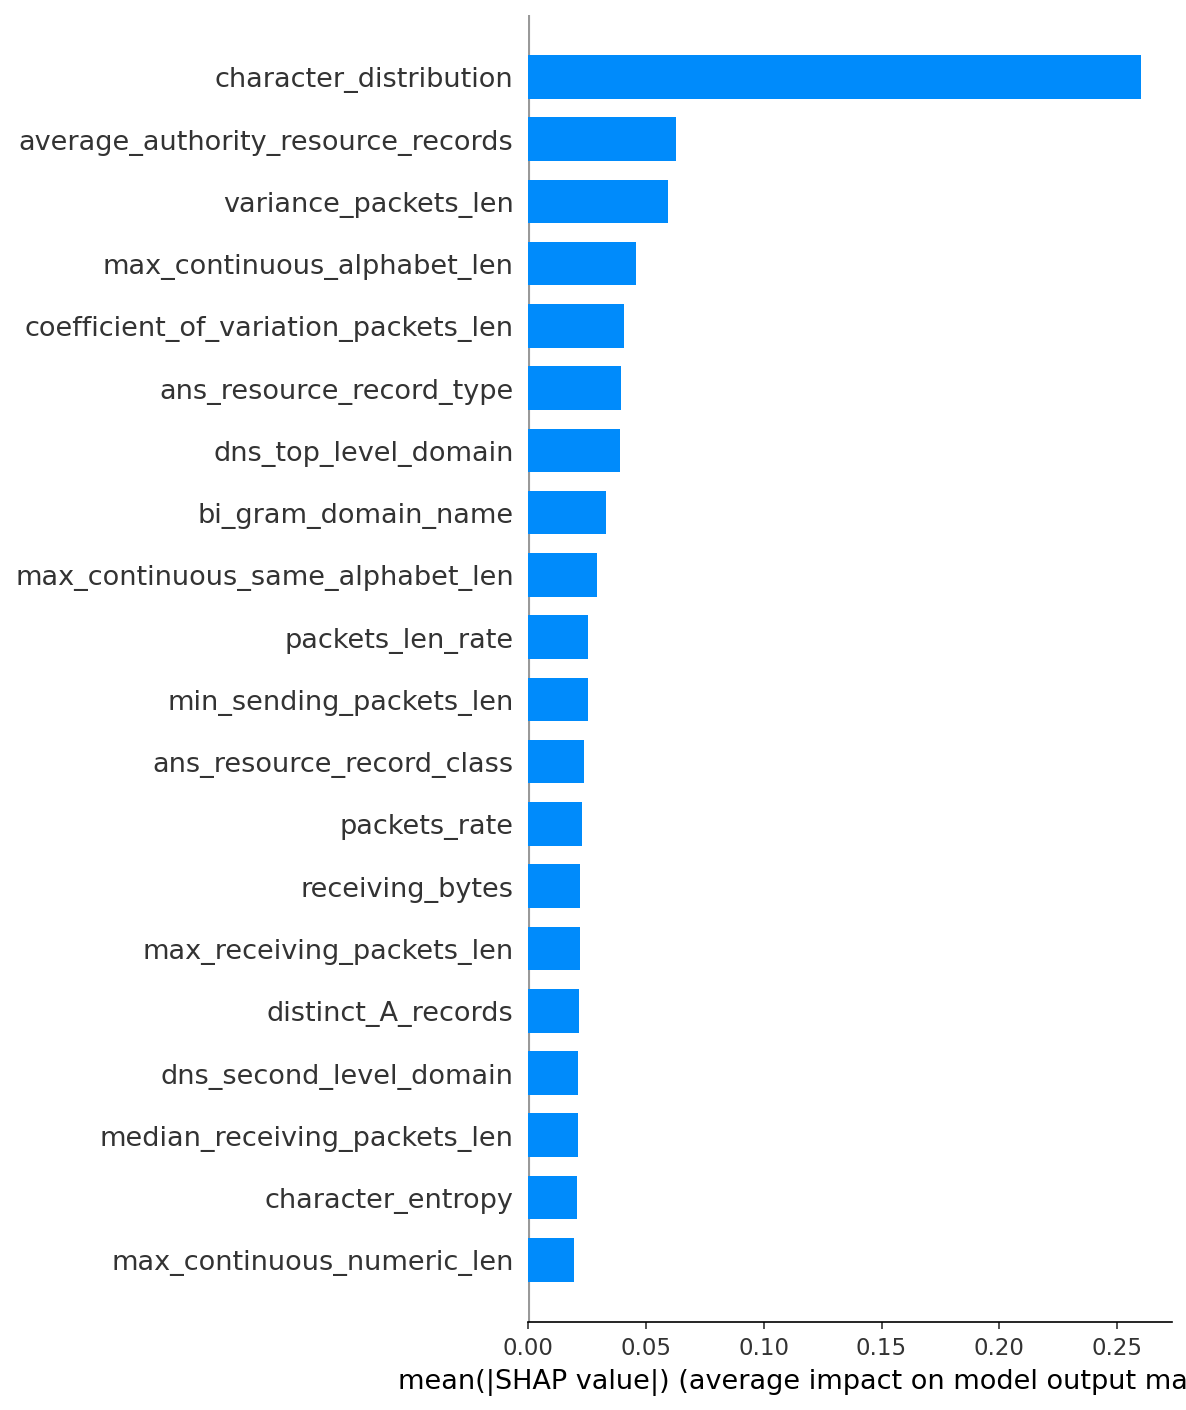
\includegraphics[width=0.75\textwidth]{figuras/shap_bar_plot-depois_sem_src_port_balanceado.png}
\caption{Importância das \textit{features} (SHAP) depois da remoção da \texttt{src\_port}, com balanceamento de classes -- modelo internacional.}
\label{fig:shap-balanceado}
\end{figure}

\section**{Especialização do modelo para domínios brasileiros (.br)}
\label{sec:especializacao-br}

Dando continuidade ao diferencial proposto pelo projeto, a especialização do modelo para o contexto brasileiro, foi conduzido um experimento comparativo entre um modelo treinado exclusivamente com as amostras de domínios \texttt{.br} filtradas dentro do próprio \textit{dataset} BCCC-CIC-Bell-DNS-2024 (``modelo brasileiro'') e o modelo treinado com o \textit{dataset} internacional completo (``modelo geral''), ambos utilizando a mesma arquitetura MLP e as mesmas \textit{features} (sem \texttt{src\_port}) definidas nas etapas anteriores. Além das métricas de classificação, também foi medida a latência média de inferência por amostra. 
O subconjunto \texttt{.br} resultante dessa filtragem é consideravelmente menor do que o \textit{dataset} internacional completo, totalizando 24.607 amostras benignas e 3.104 amostras malignas (1.984 de malware, 1.076 de phishing e 44 de spam).
Os resultados, para as classificações binária e multiclasse, são apresentados nas Tabelas~\ref{tab:br-binario} e~\ref{tab:br-multiclasse}.

\begin{table}[h]
\centering
\caption{Modelo especializado em domínios .br vs. modelo geral -- classificação binária}
\label{tab:br-binario}
\footnotesize
\resizebox{\textwidth}{!}{%
\begin{tabular}{lcccccc}
\toprule
Modelo & Acurácia & Precisão & Recall & F1-Score & AUC-ROC & Latência (ms/amostra) \\
\midrule
Brasileiro (\textit{dataset} .br) & 0,9288 & 0,8083 & 0,9510 & 0,8739 & 0,9877 & 0,0153 \\
Geral (\textit{dataset} internacional) & 0,9506 & 0,8686 & 0,9539 & 0,9093 & 0,9922 & 0,0120 \\
\bottomrule
\end{tabular}%
}
\end{table}
 
\begin{table}[h]
\centering
\caption{Modelo especializado em domínios .br vs. modelo geral -- classificação multiclasse}
\label{tab:br-multiclasse}
\footnotesize
\resizebox{\textwidth}{!}{%
\begin{tabular}{lcccccc}
\toprule
Modelo & Acurácia & Precisão & Recall & F1-Score & AUC-ROC & Latência (ms/amostra) \\
\midrule
Brasileiro (\textit{dataset} .br) & 0,9146 & 0,9227 & 0,9146 & 0,9173 & 0,9866 & 0,0169 \\
Geral (\textit{dataset} internacional) & 0,9272 & 0,9317 & 0,9272 & 0,9282 & 0,9887 & 0,0132 \\
\bottomrule
\end{tabular}%
}
\end{table}


Os resultados mostram que o modelo brasileiro apresentou desempenho ligeiramente inferior ao modelo geral em todas as métricas, tanto na tarefa binária quanto na multiclasse, o que é esperado dado o volume bem menor de amostras \texttt{.br} disponíveis no \textit{dataset} original em comparação ao conjunto internacional completo. Ainda assim, a diferença entre os dois modelos foi pequena (inferior a três pontos percentuais na maioria das métricas), o que indica que um modelo especializado é viável e mantém desempenho competitivo mesmo treinado com uma fração reduzida dos dados. Por se tratar de uma filtragem de amostras \texttt{.br} dentro de um \textit{dataset} de origem majoritariamente internacional, e não de um \textit{dataset} coletado nativamente sobre tráfego e domínios brasileiros, este resultado é interpretado como uma primeira evidência da viabilidade da especialização, sendo a coleta de um \textit{dataset} genuinamente brasileiro um passo natural para trabalhos futuros (Capítulo~\ref{cap:conclusao}).

A Figura~\ref{fig:shap-br} apresenta a explicabilidade (SHAP) do modelo brasileiro. Nota-se que, além de \texttt{character\_distribution} que se mantém como a \textit{feature} mais relevante, com magnitude ainda maior do que nos modelos internacionais, ganham destaque \texttt{dns\_second\_level\_domain} e estatísticas de TTL (\texttt{ttl\_values\_skewness}, \texttt{distinct\_ttl\_values}), sugerindo que padrões específicos do segundo nível do domínio e de configuração de TTL são particularmente relevantes para diferenciar tráfego benigno de malicioso no contexto de domínios \texttt{.br}.

\begin{figure}[h]
\centering
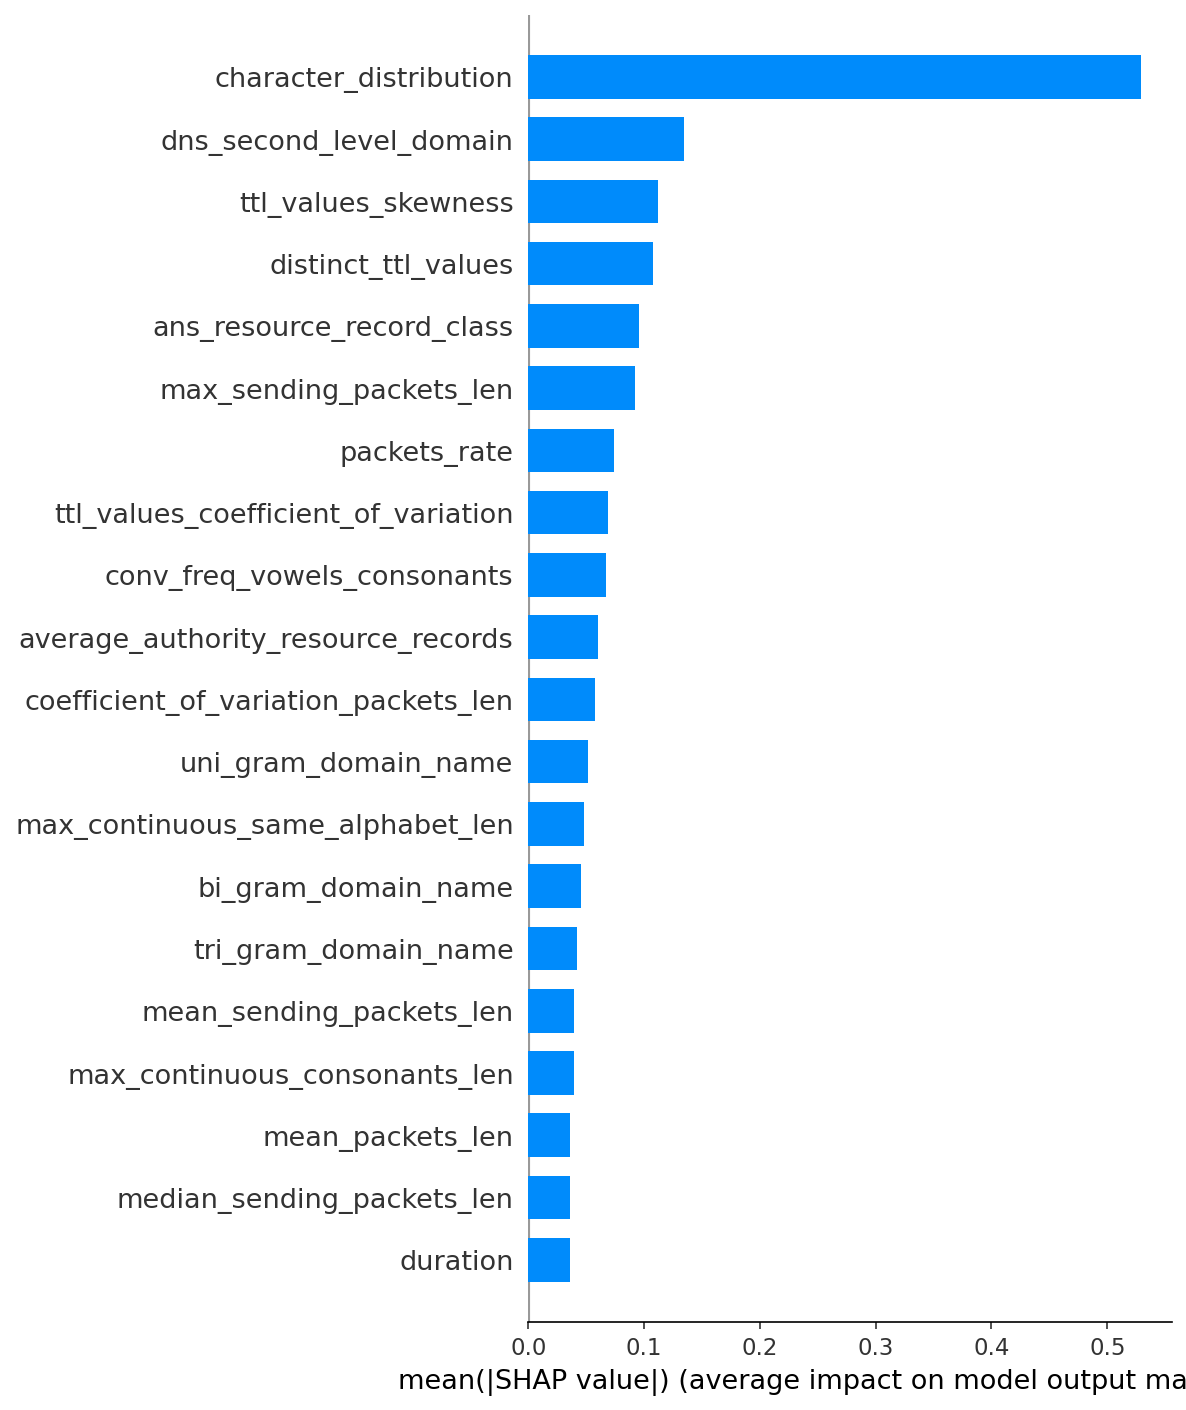
\includegraphics[width=0.75\textwidth]{figuras/shap_bar_plot_br.png}
\caption{Importância das \textit{features} (SHAP) para o modelo especializado em domínios .br.}
\label{fig:shap-br}
\end{figure}

\section**{Arquiteturas híbridas de \textit{deep learning}}

Complementando o estudo de arquiteturas (Capítulo~\ref{cap:conceitos-basicos}), foram também implementadas e avaliadas variações de arquiteturas híbridas de redes neurais profundas, combinando camadas convolucionais (CNN), recorrentes (LSTM) e densas (MLP), na forma de um \textit{ensemble} MLP+CNN+LSTM, além de outras combinações avaliadas com a mesma metodologia de pré-processamento e avaliação descrita anteriormente. Um dos resultados obtidos para a classificação binária (benigno vs. maligno) com o \textit{ensemble} MLP+CNN+LSTM é resumido na Tabela~\ref{tab:ensemble}.

\begin{table}[h]
\centering
\caption{Relatório de classificação do \textit{ensemble} MLP+CNN+LSTM (binário)}
\label{tab:ensemble}
\begin{tabular}{lcccc}
\toprule
Classe & Precisão & Recall & F1-Score & Suporte \\
\midrule
Benigno & 1,00 & 1,00 & 1,00 & 35.367 \\
Maligno & 0,46 & 0,73 & 0,57 & 126 \\
\midrule
Acurácia geral & \multicolumn{4}{c}{0,9960} \\
Média macro & 0,73 & 0,86 & 0,78 & 35.493 \\
Média ponderada & 1,00 & 1,00 & 1,00 & 35.493 \\
AUC-ROC & \multicolumn{4}{c}{0,9875} \\
\bottomrule
\end{tabular}
\end{table}

Esse experimento foi realizado sobre o conjunto de teste desbalanceado (126 amostras malignas contra 35.367 benignas), o que explica a acurácia geral e a média ponderada próximas de 1,00 mesmo com uma precisão de apenas 0,46 para a classe maligna. Ainda assim, o AUC-ROC de 0,9875 e o recall de 0,73 (0,86 na média macro) indicam boa capacidade de separação entre as classes e reforçam, junto com o experimento de balanceamento (item anterior), a importância de reportar métricas por classe, e não apenas a acurácia geral, ao avaliar modelos de IDS sobre dados desbalanceados.

\section**{Pipeline de integração para classificação em tempo real}

Como forma de aproximar o modelo desenvolvido de um cenário de uso real em produção, foi implementado um pipeline de integração que recebe um nome de domínio como entrada, realiza a captura do tráfego DNS real gerado por consultas a esse domínio, extrai as mesmas \textit{features} utilizadas no treinamento do modelo (estatísticas de TTL, tamanho e taxa de pacotes, características lexicais do nome de domínio, entre outras) e submete o vetor de \textit{features} resultante ao modelo MLP treinado, retornando a classificação do domínio (benigno ou malicioso). Esse pipeline corresponde à implementação prática dos itens 1 (captura do tráfego DNS) e 2 (classificação via aprendizado de máquina) do procedimento de mitigação descrito no artigo publicado~\citep{hirata2026dns}, faltando ainda, como trabalho futuro, a geração automática de regras de bloqueio em servidores DNS ou \textit{firewalls} a partir da classificação obtida (item 3 do procedimento).